\documentclass[11pt,oneside]{book}

\usepackage[a4paper,margin=25mm]{geometry}
\usepackage[T1]{fontenc}
\usepackage[utf8]{inputenc}
\usepackage{lmodern}
\usepackage{microtype}
\usepackage{amsmath,amssymb,bm}
\usepackage{booktabs,tabularx,array}
\usepackage{longtable}
\usepackage{graphicx}
\usepackage{xcolor}
\usepackage{enumitem}
\usepackage{listings}
\usepackage{needspace}
\usepackage{tikz}
\usetikzlibrary{arrows.meta,positioning,calc,fit,shapes.geometric}
\usepackage{fancyhdr}
\usepackage{hyperref}

\definecolor{JaxBlue}{HTML}{1261A0}
\definecolor{JaxTeal}{HTML}{138A8A}
\definecolor{JaxOrange}{HTML}{E07A1F}
\definecolor{JaxGreen}{HTML}{2E8B57}
\definecolor{JaxRed}{HTML}{B64040}
\definecolor{SoftBlue}{HTML}{EAF3FA}
\definecolor{SoftGray}{HTML}{F3F5F7}
\definecolor{CodeBg}{HTML}{F7F7F7}

\hypersetup{
  colorlinks=true,
  linkcolor=JaxBlue,
  urlcolor=JaxTeal,
  citecolor=JaxGreen!70!black,
  pdftitle={From Dynamical System to Practical Bifurcation Analysis},
  pdfauthor={JaxCont project}
}

\pagestyle{fancy}
\fancyhf{}
\fancyhead[C]{\small\color{JaxBlue}\nouppercase{\leftmark}}
\fancyfoot[C]{\thepage}
\renewcommand{\chaptermark}[1]{\markboth{\thechapter.\ #1}{}}
\renewcommand{\headrulewidth}{0.4pt}
\setlength{\headheight}{16pt}
\setlength{\headsep}{18pt}
\fancypagestyle{plain}{%
  \fancyhf{}
  \fancyfoot[C]{\thepage}
  \renewcommand{\headrulewidth}{0pt}
}
\setcounter{tocdepth}{2}
\setcounter{secnumdepth}{2}
\setlist{nosep}

\lstset{
  language=Python,
  basicstyle=\ttfamily\small,
  backgroundcolor=\color{CodeBg},
  frame=single,
  rulecolor=\color{black!20},
  keywordstyle=\color{JaxBlue}\bfseries,
  commentstyle=\color{JaxGreen!70!black},
  stringstyle=\color{JaxOrange!90!black},
  showstringspaces=false,
  columns=fullflexible,
  keepspaces=true,
  breaklines=true,
  upquote=true
}

\newcommand{\state}{\bm{u}}
\newcommand{\param}{p}
\newcommand{\R}{\mathbb{R}}
\newcommand{\residual}{F}

\newenvironment{keyidea}
  {\par\medskip\noindent\begin{minipage}{\textwidth}
   \color{JaxBlue}\rule{\textwidth}{0.8pt}\par
   \textbf{Key idea.}\ \color{black}}
  {\par\color{JaxBlue}\rule{\textwidth}{0.8pt}
   \end{minipage}\par\medskip}

\newenvironment{warningbox}
  {\par\medskip\noindent\begin{minipage}{\textwidth}
   \color{JaxRed}\rule{\textwidth}{0.8pt}\par
   \textbf{Important limitation.}\ \color{black}}
  {\par\color{JaxRed}\rule{\textwidth}{0.8pt}
   \end{minipage}\par\medskip}

\newenvironment{workflowbox}
  {\par\medskip\noindent\begin{minipage}{\textwidth}
   \color{JaxGreen!70!black}\rule{\textwidth}{0.8pt}\par
   \textbf{Research workflow.}\ \color{black}}
  {\par\color{JaxGreen!70!black}\rule{\textwidth}{0.8pt}
   \end{minipage}\par\medskip}

\newenvironment{diagnosticbox}
  {\par\medskip\noindent\begin{minipage}{\textwidth}
   \color{JaxOrange!90!black}\rule{\textwidth}{0.8pt}\par
   \textbf{Diagnostic.}\ \color{black}}
  {\par\color{JaxOrange!90!black}\rule{\textwidth}{0.8pt}
   \end{minipage}\par\medskip}

\newenvironment{trythis}
  {\par\medskip\noindent\begin{minipage}{\textwidth}
   \color{JaxTeal}\rule{\textwidth}{0.8pt}\par
   \textbf{Try it.}\ \color{black}}
  {\par\color{JaxTeal}\rule{\textwidth}{0.8pt}
   \end{minipage}\par\medskip}

\newenvironment{futurebox}
  {\par\medskip\noindent\begin{minipage}{\textwidth}
   \color{black!55}\rule{\textwidth}{0.8pt}\par
   \textbf{Future-version placeholder.}\ \color{black}}
  {\par\color{black!55}\rule{\textwidth}{0.8pt}
   \end{minipage}\par\medskip}

\title{\Huge From Dynamical System to\\[2mm]Practical Bifurcation Analysis\\[7mm]
       \Large A beginner-friendly workflow with JaxCont}
\author{JaxCont project}
\date{v0.2 tutorial edition: equilibria, periodic orbits, and JAX workflows}

\begin{document}

\frontmatter
\maketitle
\clearpage
\setcounter{page}{2}

\chapter*{About this edition}
\addcontentsline{toc}{chapter}{About this edition}
\markboth{About this edition}{}

This handbook answers a practical question:

\begin{quote}
\emph{Given a new nonlinear dynamical system, what should I compute first,
what comes next, how do I check the result, and when should I stop?}
\end{quote}

The method is broadly applicable to continuation packages, while executable
examples use JaxCont v0.2. This edition covers two supported numerical
workflows:

\begin{enumerate}
  \item continuation of equilibria with natural or pseudo-arclength methods,
        equilibrium eigenvalues, and fold/Hopf event screening;
  \item fixed-mesh collocation continuation of periodic orbits, Floquet
        stability, and fold-of-cycles, period-doubling, or Neimark--Sacker
        event screening.
\end{enumerate}

The guide deliberately goes beyond a list of API calls. Each practical chapter
states what mathematical object is being computed, how to initialize it, what
output should be inspected, how the computation commonly fails, and what
evidence is needed before a result becomes a scientific claim.

\begin{warningbox}
Do not infer software support from a design document, internal scaffold, or
class name. Branch switching, automatic cycle initialization from a Hopf point,
adaptive periodic meshes, two-parameter continuation, codimension-two
classification, and global-orbit continuation remain future work. They are
kept as explicit placeholders so this guide can grow without pretending those
commands already exist.
\end{warningbox}

\section*{Capability map for this edition}

\begin{tabularx}{\textwidth}{>{\bfseries}p{.25\textwidth}p{.20\textwidth}X}
\toprule
Workflow & Status & Where to learn it\\
\midrule
Equilibrium continuation & Supported & Chapters~4--10 and Examples 01--07\\
Equilibrium fold/Hopf screening & Supported, eager events & Chapters~6--10\\
Periodic-orbit collocation & Supported & Chapter~12 and Examples 10--11\\
Floquet stability, PD, NS & Supported & Chapter~12 and Examples 08--09\\
Branch switching & Future & Chapter~11 placeholder\\
Two-parameter/global analysis & Future & Chapter~13 placeholder\\
\bottomrule
\end{tabularx}

\chapter*{How to use this book}
\addcontentsline{toc}{chapter}{How to use this book}
\markboth{How to use this book}{}

The book is cumulative, but it supports several routes:

\begin{description}
  \item[First continuation run.] Read Chapters~1--7, then reproduce the scalar
        fold case study before adapting the code to a new model.
  \item[Existing equilibrium model.] Begin with the model worksheet and
        starting-root checks in Chapters~4--5, then use Chapters~6--9 as an
        execution and validation checklist.
  \item[Periodic orbit.] Read the stability distinction in Chapter~2 and the
        equilibrium workflow once, then follow Chapter~12 in order.
  \item[JAX study.] After one validated scalar run, use the ensemble and
        differentiability material in Chapters~9--10.
\end{description}

Code blocks are meant to be run, not merely read. Lines marked as diagnostics
should be retained in research scripts until the workflow is stable. Values in
the examples are starting points, not universal tolerances.

\tableofcontents

\mainmatter

\part{Foundations}

\chapter{What bifurcation analysis computes}

\section{A dynamical system and its equilibria}

Consider an autonomous system
\[
  \dot{\state}=f(\state,\param;\theta),
  \qquad \state\in\R^n,
\]
where $\param$ is the parameter to be varied and $\theta$ contains fixed model
parameters. An equilibrium is a state $\state^*$ satisfying
\[
  f(\state^*,\param;\theta)=0.
\]
For numerical work it is useful to call the right-hand side a residual,
\[
  \residual(\state,\param)=f(\state,\param;\theta).
\]

A single root solve finds one pair $(\state^*,\param)$. Continuation follows a
connected curve of such pairs while the parameter changes.

\section{Four computations that are easy to confuse}

The same model can appear in four different numerical tasks:

\begin{description}
  \item[Time integration] fixes parameters and advances an initial state in
        physical time. It answers ``where does this trajectory go?''
  \item[Root solving] fixes the parameter and solves $F(\state,p)=0$. It
        answers ``is there an equilibrium near this initial guess?''
  \item[Continuation] starts from one verified solution and follows a connected
        family. It answers ``how does this solution change with a parameter?''
  \item[Event refinement] starts from a sign-changing bracket on a branch and
        solves a more specialized local problem. It answers ``where precisely
        does this fold or spectral crossing occur?''
\end{description}

These tasks support one another but are not interchangeable. Simulation is
often the easiest way to obtain an initial cycle, while continuation is the
tool that can retain unstable solutions that simulation will not approach.

\begin{keyidea}
Simulation follows a state through physical time. Continuation follows a family
of mathematical solutions through state--parameter space. They answer different
questions and should be used together.
\end{keyidea}

\section{One continuation interface, two residual meanings}

JaxCont's continuation engine sees a square residual $F(U,p)=0$. The meaning
of $U$ depends on the problem:

\noindent\begin{tabularx}{\textwidth}{>{\bfseries}p{.25\textwidth}p{.31\textwidth}X}
\toprule
Problem kind & Unknown $U$ & Residual meaning\\
\midrule
Equilibrium & physical state $\state$ & ODE right-hand side
$f(\state,p)$\\
Periodic orbit & mesh states, collocation states, period $T$ & collocation
defects, interval continuity, and one phase condition\\
\bottomrule
\end{tabularx}

This is the central v0.2 design idea: periodic-orbit continuation does not need
a second branch-following algorithm. It needs a factory that turns an entire
cycle into a finite-dimensional root problem. Natural or pseudo-arclength
continuation can then operate on that larger residual.

\section{What a bifurcation diagram means}

A bifurcation diagram normally places a parameter on the horizontal axis and
one chosen state observable on the vertical axis. Each point represents an
equilibrium, not a time sample. Stable and unstable segments describe local
behavior near those equilibria.

\begin{center}
\begin{tikzpicture}[x=1.7cm,y=1.05cm,>=Latex]
  \draw[->] (-2.8,0)--(2.8,0) node[right] {$p$};
  \draw[->] (0,-2.5)--(0,2.5) node[above] {observable};
  \draw[JaxBlue,very thick,smooth,domain=-2.05:2.05,samples=100]
      plot ({\x^3/3-\x},{\x});
  \foreach \x in {-1.8,-1.3,-.8,-.3,.2,.7,1.2,1.7}
    \fill[JaxOrange] ({\x^3/3-\x},{\x}) circle (1.5pt);
  \node[align=left,anchor=west] at (1.05,1.75)
      {one connected\\solution branch};
\end{tikzpicture}
\end{center}

\section{The questions continuation can answer}

\begin{tabularx}{\textwidth}{>{\raggedright\arraybackslash}p{.30\textwidth}X}
\toprule
Question & Useful output\\
\midrule
Where do steady states exist? & Equilibrium branches over a parameter range.\\
Can several steady states coexist? & Multiple branch segments at the same
parameter value.\\
Where may abrupt transitions occur? & Fold candidates and stability changes.\\
Where can oscillatory instability begin? & Hopf candidates on equilibrium
branches.\\
How robust is the diagram? & Repeated branches over uncertain parameters or
model variants.\\
\bottomrule
\end{tabularx}

\begin{warningbox}
A computed diagram describes the supplied mathematical model. It does not by
itself establish causality, estimate parameters, prove that every solution has
been found, or validate the model against observations.
\end{warningbox}

\begin{trythis}
For a diagram in your field, write one sentence for each axis, one sentence for
what a point represents, and one sentence for what stability means. If you
cannot do this without saying ``the simulation,'' return to the distinction
between trajectory time and branch progress.
\end{trythis}

\chapter{Stability and local bifurcations}

\section{Linearization}

Near an equilibrium, write $\state=\state^*+\delta\state$. To first order,
\[
  \dot{\delta\state}=J\,\delta\state,
  \qquad
  J=\frac{\partial f}{\partial\state}(\state^*,\param).
\]
The eigenvalues $\lambda_i$ of $J$ determine local equilibrium stability:

\begin{itemize}
  \item if every $\operatorname{Re}\lambda_i<0$, the equilibrium is locally
        asymptotically stable;
  \item if any $\operatorname{Re}\lambda_i>0$, it is unstable;
  \item if an eigenvalue is close to the imaginary axis, the linear test is
        sensitive and a bifurcation may be nearby.
\end{itemize}

\subsection{Worked example: the Van der Pol equilibrium}

For
\[
  \dot x=y,\qquad \dot y=\mu(1-x^2)y-x,
\]
the origin is an equilibrium for every $\mu$. Its Jacobian is
\[
  J(0,0;\mu)=\begin{bmatrix}0&1\\-1&\mu\end{bmatrix},
\]
with characteristic equation
\[
  \lambda^2-\mu\lambda+1=0.
\]
For $\mu<0$ both eigenvalues have negative real part; for $\mu>0$ both have
positive real part; at $\mu=0$ they are $\pm i$. This analytic calculation
provides three checks for software:

\begin{enumerate}
  \item the equilibrium branch should remain exactly at $(x,y)=(0,0)$;
  \item the stability flag should change at $\mu=0$;
  \item a Hopf event test should be bracketed near $\mu=0$.
\end{enumerate}

The third statement is only a candidate classification. In this particular
example the first Lyapunov coefficient is zero, so the crossing is degenerate.
The example is valuable precisely because it teaches that a correct spectral
crossing is not the same as a generic Hopf theorem.

\section{Common local equilibrium bifurcations}

\begin{tabularx}{\textwidth}{>{\bfseries}p{.20\textwidth}p{.26\textwidth}X}
\toprule
Type & Linear signature & Interpretation\\
\midrule
Fold (LP) & one real eigenvalue reaches zero & two equilibrium branches meet
and turn; multistability may begin or end\\
Hopf (H) & a complex-conjugate pair reaches the imaginary axis & equilibrium
stability changes and a family of periodic orbits may be present\\
Pitchfork & zero eigenvalue plus symmetry/normal-form conditions & a symmetric
branch meets two symmetry-related branches\\
Transcritical & zero eigenvalue plus branch-intersection conditions & two
equilibrium branches intersect and exchange stability\\
\bottomrule
\end{tabularx}

\begin{warningbox}
An eigenvalue crossing is a candidate condition, not a complete classification.
Pitchfork and transcritical bifurcations need structural information; a generic
Hopf classification needs nondegeneracy information such as a first Lyapunov
coefficient. Current JaxCont event detection reports fold and Hopf candidates.
\end{warningbox}

\section{Global and periodic-orbit bifurcations}

Period doubling, torus bifurcations, folds of cycles, homoclinic orbits,
heteroclinic connections, and SNIC bifurcations involve periodic or global
objects rather than only the local equilibrium Jacobian. They require
additional representations, test functions, and solvers.

JaxCont v0.2 supports fixed-mesh periodic-orbit collocation, Floquet
multipliers, folds of cycles through the tangent-based fold test, period
doubling, and Neimark--Sacker screening. Homoclinic, heteroclinic, SNIC, and
other global-orbit workflows remain future work.

\noindent\begin{tabularx}{\textwidth}{>{\bfseries}p{.26\textwidth}p{.27\textwidth}X}
\toprule
Solution type & Stability object & Typical crossing\\
\midrule
Equilibrium & eigenvalues $\lambda$ of $f_{\state}$ &
$\operatorname{Re}\lambda=0$\\
Periodic orbit & Floquet multipliers $\mu$ of the one-period map &
$|\mu|=1$ after excluding the trivial multiplier near $+1$\\
\bottomrule
\end{tabularx}

\begin{warningbox}
Do not apply the negative-real-part rule to Floquet multipliers. Equilibrium
eigenvalues are continuous-time growth rates; Floquet multipliers are
one-period growth factors. Their stability criteria are different.
\end{warningbox}

\chapter{Why continuation is needed}

\section{A parameter sweep is not continuation}

A simulation sweep selects parameter values, simulates from chosen initial
conditions, and records the long-time behavior. It may miss unstable
equilibria, depend strongly on initial conditions, and jump between attractors.
Continuation instead uses the preceding solution as information for the next
one and can follow unstable equilibrium segments.

\subsection{A concrete failure of a sweep}

For $F(x,r)=r-x^2$, the equilibria are $x=\pm\sqrt r$ for $r\ge0$. A simulation
started near the positive state will normally reveal only the attracting
solution compatible with that initial condition. A root sweep initialized from
the previous positive root can approach $r=0$ but has no instruction for
turning onto the negative branch. The missing branch is not absent from the
equations; it is absent from the workflow.

\section{Natural parameter continuation}

At an accepted point $(\state_k,p_k)$, natural continuation predicts a new
parameter $p_{k+1}=p_k+\Delta p$ and solves
\[
  \residual(\state,p_{k+1})=0
\]
for $\state$. It is simple and effective while the branch is a single-valued
function $\state(p)$.

Differentiate the equilibrium equation:
\[
  \residual_{\state}\frac{d\state}{dp}+\residual_p=0,
  \qquad
  \frac{d\state}{dp}=-\residual_{\state}^{-1}\residual_p.
\]
At a fold, $\residual_{\state}$ becomes singular. Decreasing the parameter step
can approach the fold but does not change this geometry.

\begin{lstlisting}
def quadratic_rhs(u, r, args):
    return jnp.array([r - u[0] ** 2])

problem = jc.bif_problem(
    quadratic_rhs, u0=jnp.array([1.0]), p0=1.0
)

natural = jc.continuation(
    problem, jc.Natural(), p_span=(1.0, -1.0),
    settings=jc.ContinuationPar(
        ds=0.05, max_steps=30,
        newton_tol=1e-6, newton_max_iter=50,
    ),
)
\end{lstlisting}

The target $r=-1$ intentionally lies beyond the fold even though no real
equilibrium exists there. The informative output is not a ``failed physics''
claim; it is that natural continuation stalls before $r=0$ because each
corrector keeps $r$ fixed.

\section{Pseudo-arclength continuation}

Pseudo-arclength introduces an artificial curve coordinate $s$ and treats both
$\state$ and $p$ as unknowns. With unit tangent
$\bm{t}_k=(\dot{\state}_k,\dot p_k)$, predict
\[
  (\state_{\mathrm{pred}},p_{\mathrm{pred}})
  =(\state_k,p_k)+\Delta s\,\bm{t}_k.
\]
Then solve
\[
\begin{cases}
\residual(\state,p)=0,\\
(\state-\state_k)^T\dot{\state}_k+
(p-p_k)\dot p_k-\Delta s=0.
\end{cases}
\]

\begin{center}
\begin{tikzpicture}[x=1.55cm,y=1.0cm,>=Latex]
  \draw[->] (-2.5,0)--(2.8,0) node[right] {$p$};
  \draw[->] (0,-2.35)--(0,2.35) node[above] {$u$};
  \draw[JaxBlue,very thick,smooth,domain=-2:2,samples=100]
      plot ({\x^3/3-\x},{\x});
  \coordinate (old) at (.375,-1.50);
  \coordinate (pred) at (1.00,-1.00);
  \coordinate (new) at (.645,-.85);
  \fill[JaxBlue] (old) circle (2.5pt) node[below left] {accepted};
  \draw[JaxOrange,very thick,->] (old)--(pred);
  \fill[JaxOrange] (pred) circle (2.5pt) node[below right] {predicted};
  \draw[JaxGreen,dashed,thick] ($(new)!-.65!(pred)$)--($(new)!1.65!(pred)$);
  \draw[JaxGreen,very thick,->] (pred)--(new);
  \fill[JaxGreen!75!black] (new) circle (2.5pt) node[above left] {corrected};
\end{tikzpicture}
\end{center}

One Newton correction solves the bordered system
\[
\begin{bmatrix}
\residual_{\state} & \residual_p\\
\dot{\state}_k^T & \dot p_k
\end{bmatrix}
\begin{bmatrix}\delta\state\\\delta p\end{bmatrix}
=-
\begin{bmatrix}\residual(\state,p)\\g(\state,p)\end{bmatrix}.
\]
Although $\residual_{\state}$ is singular at an ordinary fold, the full
bordered matrix can remain nonsingular.

\subsection{Run the same problem with pseudo-arclength}

\begin{lstlisting}
palc = jc.continuation(
    problem, jc.PseudoArclength(), p_span=(1.0, -1.0),
    settings=jc.ContinuationPar(
        ds=0.05, max_steps=60,
        newton_tol=1e-6, newton_max_iter=50,
    ),
)

print(palc.branch.params[-1], palc.branch.states[-1, 0])
\end{lstlisting}

After reaching the fold, the parameter turns back toward positive values while
the state moves onto $x<0$. Therefore the endpoint $-1$ is not a literal
destination that must be reached after the turn; it sets the initial
orientation. Inspect the ordered $(r,x)$ pairs rather than judging success only
from the final parameter.

\begin{diagnosticbox}
If pseudo-arclength also stops early, inspect the starting residual, accepted
point count, step sizes, non-finite values, Newton tolerance, and attempt
budget. ``The branch ends here'' is the last interpretation, not the first.
\end{diagnosticbox}

\part{The practical JaxCont workflow}

\chapter{Step 1: understand and encode the model}

\section{Model worksheet}

Before writing continuation code, record:

\begin{enumerate}
  \item state variables, units, and physically meaningful ranges;
  \item fixed parameters and their provenance;
  \item the proposed continuation parameter and a defensible range;
  \item which state or derived observable should appear in the diagram;
  \item expected symmetries, invariants, discontinuities, and singularities;
  \item whether the scientific question concerns equilibria or time-dependent
        solutions.
\end{enumerate}

\begin{workflowbox}
Choose one continuation parameter first. A two-parameter scientific question
can often begin as several one-parameter slices. This is easier to debug and is
compatible with the one-parameter continuation workflow. A batch of such slices
is useful exploration, but it is not the same as continuing a bifurcation point
in two parameters.
\end{workflowbox}

\subsection{A model worksheet example}

For the Brusselator,
\[
  \dot x=a-(b+1)x+x^2y,\qquad
  \dot y=bx-x^2y,
\]
one useful worksheet is:

\noindent\begin{tabularx}{\textwidth}{>{\bfseries}p{.25\textwidth}X}
\toprule
Item & Decision\\
\midrule
State & $(x,y)$, both expected to remain non-negative\\
Fixed parameter & $a=1$\\
Continuation parameter & $b$\\
Equilibrium question & stability change near $b=1+a^2=2$\\
Periodic question & cycle amplitude and period for $b>2$\\
Observable & equilibrium $x$; for cycles, peak-to-peak $x$ amplitude and $T$\\
Independent check & time integration and the analytic Hopf threshold\\
\bottomrule
\end{tabularx}

This worksheet separates two solution objects before any software is called.
The equilibrium branch and the periodic branch require different starts,
stability objects, and plots.

\section{The JaxCont residual signature}

JaxCont expects a function of state, continuation parameter, and fixed
arguments:

\begin{lstlisting}
def rhs(u, p, args):
    # u: state vector
    # p: scalar continuation parameter
    # args: fixed parameters or other JAX PyTree data
    return residual_vector
\end{lstlisting}

Use \texttt{jax.numpy} operations and return a one-dimensional array with the
same number of residual equations as state variables. Keep the function smooth
where possible. Hard clipping, conditionals, lookup discontinuities, and
non-finite expressions can make Newton correction and automatic
differentiation unreliable.

\subsection{Put fixed model data in \texttt{args}}

\begin{lstlisting}
def lorenz84_rhs(u, forcing, args):
    X, Y, Z, U = u
    alpha, beta, gamma, delta, G, T = args

    return jnp.array([
        -Y**2 - Z**2 - alpha*X + alpha*forcing - gamma*U**2,
        X*Y - beta*X*Z - Y + G,
        beta*X*Y + X*Z - Z,
        -delta*U + gamma*U*X + T,
    ])
\end{lstlisting}

Here \texttt{forcing} is the scalar continuation parameter and the remaining
constants form a tuple in \texttt{args}. This distinction matters later:
\texttt{problem.at(args=...)} is the natural axis for a \texttt{vmap} ensemble
or a sensitivity calculation.

\subsection{Residual patterns to avoid}

\begin{tabularx}{\textwidth}{>{\ttfamily}p{.31\textwidth}X}
\toprule
\normalfont Pattern & Why it is dangerous\\
\midrule
if u[0] > 0: & Python branching on a traced value fails under JAX transforms;
use a smooth model or array control where mathematically appropriate.\\
numpy.sin(u) & Host NumPy can copy data out of the JAX program; use
\texttt{jax.numpy}.\\
jnp.clip(...), abs(...) & Nonsmooth points can make Newton derivatives
misleading even when the code traces.\\
1 / (u[0] - c) & A branch approaching the pole can produce non-finite
residuals and terminate the solver.\\
global mutable data & Compilation assumes the traced function is effectively
pure; hidden mutation makes behavior difficult to reason about.\\
\bottomrule
\end{tabularx}

\begin{trythis}
Evaluate your residual at the initial state, at a small perturbation, and under
\texttt{jax.jacfwd}. Check shape, dtype, finite values, and whether the
Jacobian changes smoothly. This catches many model-encoding problems before
continuation adds another layer of complexity.
\end{trythis}

\chapter{Step 2: find and verify a starting equilibrium}

\section{Why the starting point matters}

Continuation does not discover a branch from nothing. It requires a pair
$(\state_0,p_0)$ satisfying
\[
  \|\residual(\state_0,p_0)\|\ll1.
\]
An approximate point from simulation, an analytic equilibrium, experimental
knowledge, or a separate root solver is acceptable only after residual
verification.

\begin{lstlisting}
residual = rhs(u0, p0, args)
residual_norm = jnp.linalg.norm(residual, ord=jnp.inf)
print("starting residual:", float(residual_norm))
\end{lstlisting}

\begin{warningbox}
\texttt{p\_span[0]} is the literal parameter paired with
\texttt{problem.u0} when continuation begins. It must describe the same
equilibrium as the supplied state. Storing a different value in
\texttt{problem.p0} does not repair an inconsistent starting pair.
\end{warningbox}

\section{Three ways to obtain a start}

\subsection{Use an analytic equilibrium}

For $F(x,p)=p+x-x^3/3$, choose any $x_0$ and compute
$p_0=x_0^3/3-x_0$. With $x_0=-2$, the consistent parameter is
$p_0=-2/3$. Writing $p_0=-1$ because it is a convenient plot boundary would
create an inconsistent pair.

\subsection{Refine a simulation or hand estimate}

The neural-mass gallery example uses the package's Newton solver:

\begin{lstlisting}
from jaxcont.solvers.newton import NewtonSolver

guess = jnp.array([0.238616, 0.982747, 0.367876])
p0 = -2.0
r0 = jnp.linalg.norm(rhs(guess, p0, args))

solver = NewtonSolver(tol=1e-5, max_iter=100)
u0, converged, n_iter = solver.solve(
    lambda u: rhs(u, p0, args), guess
)

check = jnp.linalg.norm(rhs(u0, p0, args), ord=jnp.inf)
print(converged, n_iter, float(check))
\end{lstlisting}

Keep the final explicit residual check even when \texttt{converged} is true.
The example uses $10^{-5}$ rather than assuming that $10^{-8}$ is reachable
for a stiff float32 problem.

\subsection{Load a trusted reference point}

A point from another continuation package or a previous run can be an excellent
start if equations, parameter ordering, scaling, precision, and units match.
Always reevaluate the current residual after loading it. A copied state is data,
not proof that it belongs to the current model.

\section{How to search for multiple equilibria}

A single root solve normally returns a single root. To investigate
multistability:

\begin{enumerate}
  \item generate several physically plausible initial guesses;
  \item solve at the same parameter value;
  \item reject roots with large residuals or invalid state values;
  \item cluster nearly identical roots;
  \item continue each distinct verified root;
  \item compare the resulting connected branches.
\end{enumerate}

Failure to find another root is not proof that none exists.

\begin{lstlisting}
guesses = jnp.linspace(-3.0, 3.0, 25)
roots = []

for guess in guesses:
    u, ok, _ = solver.solve(
        lambda z: rhs(z, p0, args),
        jnp.array([guess]),
    )
    if ok and jnp.linalg.norm(rhs(u, p0, args)) < 1e-5:
        roots.append(float(u[0]))

# Cluster only after checking physical admissibility and residuals.
unique_roots = []
for root in sorted(roots):
    if not unique_roots or abs(root - unique_roots[-1]) > 1e-4:
        unique_roots.append(root)
\end{lstlisting}

\begin{warningbox}
A dense grid of initial guesses is a search strategy, not a completeness
theorem. Closely spaced roots, high-dimensional basins of convergence, and
constraints can still hide solutions.
\end{warningbox}

\chapter{Steps 3--5: continue, assess stability, and detect events}

\section{A complete minimal run}

\begin{lstlisting}
import jax.numpy as jnp
import jaxcont as jc

def rhs(u, p, args):
    x = u[0]
    return jnp.array([p + x - x**3 / 3])

problem = jc.bif_problem(
    rhs,
    u0=jnp.array([-2.0]),
    p0=-2.0 / 3.0,
    state_names=["x"],
    param_name="p",
)

settings = jc.ContinuationPar(
    ds=0.01,
    ds_min=1e-5,
    ds_max=0.05,
    max_steps=300,
    newton_tol=1e-6,
    newton_max_iter=20,
    compute_stability=True,
)

result = jc.continuation(
    problem,
    jc.PseudoArclength(),
    p_span=(-2.0 / 3.0, 1.0),
    settings=settings,
    events=[jc.Fold()],
)
\end{lstlisting}

Before running, verify the exact relation:

\begin{lstlisting}
start_residual = rhs(problem.u0, -2.0 / 3.0, None)
assert float(jnp.linalg.norm(start_residual)) < 1e-6
\end{lstlisting}

This scalar model has only real eigenvalues, so requesting \texttt{Hopf()} would
add no useful information. Event lists should reflect the model and branch
kind, not a boilerplate copied from another script.

\section{How to read the result}

The high-level result contains:

\begin{itemize}
  \item \texttt{result.branch.states}: accepted state vectors;
  \item \texttt{result.branch.params}: corresponding parameter values;
  \item stability/eigenvalue information when requested;
  \item \texttt{result.events}: detected fold or Hopf candidates;
  \item \texttt{result.stats}: run summary information.
\end{itemize}

In an ordinary eager call, branch arrays are trimmed to the accepted points.
Inside \texttt{jax.jit} or \texttt{jax.vmap}, fixed buffers and a validity mask
are returned because transformed JAX code needs predictable shapes.

\subsection{Inspect before plotting}

\begin{lstlisting}
branch = result.branch

print("accepted points:", branch.n_valid)
print("parameter range:",
      float(branch.params.min()), float(branch.params.max()))
print("last point:", branch.params[-1], branch.states[-1])

for event in result.events:
    print(event.kind, event.p, event.u)
\end{lstlisting}

The last point alone is not a termination diagnosis. A pseudo-arclength branch
can turn away from the requested endpoint, and a failed attempt can consume the
attempt budget without creating an output point. Compare the ordered
parameters, states, and step-size diagnostics.

\section{Choosing numerical settings}

\begin{tabularx}{\textwidth}{>{\ttfamily}p{.24\textwidth}X}
\toprule
\normalfont Setting & Interpretation\\
\midrule
ds & initial distance for the next prediction\\
ds\_min & smallest permitted retry step; reaching it can stop the run\\
ds\_max & largest adaptive step; smaller values give denser branch sampling\\
max\_steps & attempt budget, including failed retries\\
newton\_tol & correction convergence tolerance\\
newton\_max\_iter & maximum Newton iterations per attempt\\
compute\_stability & whether equilibrium eigenvalues are computed\\
\bottomrule
\end{tabularx}

Begin conservatively. If the branch is smooth and corrections are easy, allow
adaptive growth. Near sharp turns, close events, or stiff regions, reduce
\texttt{ds\_max} and verify that conclusions persist.

\subsection{A tuning sequence}

\begin{enumerate}
  \item Start with a verified root, moderate \texttt{ds}, generous
        \texttt{max\_steps}, and no events.
  \item Confirm that the branch moves in the intended initial direction.
  \item Enable stability and inspect the spectrum at a few points.
  \item Add events only after branch and spectra are credible.
  \item Reduce \texttt{ds\_max} near important events and repeat.
  \item Tighten \texttt{newton\_tol} only while residual reduction continues;
        do not demand a value beneath the dtype/problem precision floor.
\end{enumerate}

\begin{diagnosticbox}
If every attempted step is rejected, a smaller \texttt{ds} may help, but first
check the starting root and tolerance. A tolerance below the attainable
float32 residual floor makes adaptive step size collapse even when the
mathematical branch is smooth.
\end{diagnosticbox}

\section{Natural or pseudo-arclength?}

\begin{tabularx}{\textwidth}{p{.27\textwidth}XX}
\toprule
 & \texttt{Natural()} & \texttt{PseudoArclength()}\\
\midrule
Correction unknowns & state only & state and parameter\\
At an ordinary fold & normally stalls & can continue through\\
Cost per Newton step & $n\times n$ solve & $(n+1)\times(n+1)$ solve\\
Recommended use & simple monotone reference branch & exploratory
bifurcation analysis\\
\bottomrule
\end{tabularx}

\section{Event detection is a screening step}

Fold and Hopf events should be treated as candidates:

\begin{enumerate}
  \item identify the bracket or reported location;
  \item inspect nearby eigenvalues and residuals;
  \item repeat with a smaller step bound;
  \item refine with an appropriate local solve when available;
  \item check model-specific nondegeneracy or symmetry conditions;
  \item compare important events with an analytic result or another tool.
\end{enumerate}

\subsection{Use events on the correct solution kind}

\begin{tabularx}{\textwidth}{>{\ttfamily}p{.27\textwidth}p{.25\textwidth}X}
\toprule
\normalfont Event & Branch kind & Test idea\\
\midrule
Fold() & equilibrium or periodic & parameter component of the branch tangent\\
Hopf() & equilibrium & real part of a genuinely complex eigenvalue pair\\
PeriodDoubling(...) & periodic & nontrivial real multiplier crosses $-1$\\
NeimarkSacker(...) & periodic & complex multiplier pair crosses the unit circle\\
\bottomrule
\end{tabularx}

JaxCont v0.2 does not yet reject every kind mismatch. A
\texttt{PeriodDoubling} event on equilibrium eigenvalues or a \texttt{Hopf}
event on Floquet multipliers may execute but has no valid mathematical meaning.

\begin{diagnosticbox}
Event detection runs on the eager result path because bracketing, sorting, and
deduplication use Python-level orchestration. Do not request events inside
\texttt{jax.vmap} or an outer \texttt{jax.jit}; batch branch/stability arrays
first and screen selected runs afterwards.
\end{diagnosticbox}

\chapter{Step 6: interpret and visualize the branch}

\section{Choose an observable}

For an $n$-dimensional state, a two-dimensional plot requires a selected
component or derived quantity $h(\state)$. Choose it for scientific meaning,
not merely because it is the first state component. Useful choices include a
concentration, voltage, firing rate, norm, energy-like quantity, or maximum
component.

\subsection{Use the result convenience plot first}

\begin{lstlisting}
fig = result.plot(
    state_index=0,
    annotate=True,
    title="Scalar equilibrium branch",
)
\end{lstlisting}

For a multi-state equilibrium model, the visualization module also provides
all-state, phase-portrait, and eigenvalue helpers. The v0.2 result retains an
underlying compatibility object for utilities that still expect the older
solution representation:

\begin{lstlisting}
from jaxcont.viz import plot_all_states, plot_eigenvalues

solution = result._solution  # v0.2 compatibility bridge
fig_states = plot_all_states(solution)
fig_spectrum = plot_eigenvalues(result, show_events=True)
\end{lstlisting}

The leading underscore is a reminder that this bridge may evolve. Prefer
\texttt{result.branch} and \texttt{result.events} for new numerical analysis,
and use the plotting helpers as presentation utilities.

\section{A validated scalar fold example}

The residual
\[
  F(x,p)=p+x-\frac{x^3}{3}
\]
has branch $p=x^3/3-x$ and analytic folds at
\[
  (x,p)=(-1,2/3),\qquad(1,-2/3).
\]
It is an ideal first test because geometry, singularity, and expected event
locations are known exactly.

\begin{figure}[htbp]
\centering
\includegraphics[width=.78\textwidth]{../../examples/images/pitchfork_bifurcation.png}
\caption{Repository-generated JaxCont equilibrium branch for the scalar cubic
example. The filename retains its historical ``pitchfork'' label, but the
displayed imperfect cubic branch is used here primarily as an analytic fold
test.}
\end{figure}

\section{What not to over-interpret}

\begin{itemize}
  \item A stable equilibrium branch does not reveal its full basin of attraction.
  \item An unstable equilibrium can still organize transient dynamics.
  \item A Hopf candidate does not provide the amplitude or stability of cycles.
  \item One connected run does not guarantee discovery of disconnected branches.
  \item Plot smoothness does not guarantee small residuals or correct event labels.
\end{itemize}

\subsection{Plot the diagnostic, not only the headline}

For an equilibrium study, keep at least three views during development:

\begin{enumerate}
  \item the chosen branch observable versus parameter;
  \item the largest real part of the equilibrium spectrum versus parameter;
  \item the residual norm and step size versus accepted-point index.
\end{enumerate}

For a periodic study, replace the second view with nontrivial Floquet
multiplier magnitude and add period or amplitude. A publication figure may
show only the final observable, but the working analysis should preserve the
diagnostics that justify it.

\chapter{Step 7: validate before interpreting}

\section{The validation ladder}

\begin{center}
\begin{tikzpicture}[node distance=7mm,>=Latex,
 box/.style={rounded corners,draw=JaxBlue,fill=SoftBlue,
             minimum width=95mm,minimum height=9mm,align=center}]
\node[box] (r) {1. residuals and finite values};
\node[box,below=of r] (s) {2. repeat with changed step bounds and tolerances};
\node[box,below=of s] (d) {3. continue in both directions or from another root};
\node[box,below=of d] (a) {4. compare with analytic limits or conservation laws};
\node[box,below=of a] (t) {5. compare selected points with simulation or another tool};
\draw[->,thick] (r)--(s);
\draw[->,thick] (s)--(d);
\draw[->,thick] (d)--(a);
\draw[->,thick] (a)--(t);
\end{tikzpicture}
\end{center}

\section{Residual checks}

For every accepted point, evaluate
\[
  r_k=\|\residual(\state_k,p_k)\|_\infty.
\]
Plot or summarize $r_k$. A success flag is useful, but the physical equations
are the final numerical check.

\begin{lstlisting}
residuals = jax.vmap(
    lambda u, p: rhs(u, p, problem.args)
)(result.branch.states, result.branch.params)

residual_norms = jnp.linalg.norm(residuals, ord=jnp.inf, axis=1)
print("max accepted residual:", float(residual_norms.max()))
\end{lstlisting}

This direct equilibrium check is intentionally independent of the solver's
stored convergence flag. For periodic problems, call the assembled
\texttt{problem.f(U, p, problem.args)} in the same way; its residual includes
collocation defects, continuity, and phase error.

\section{Resolution and direction checks}

Run at least a small matrix of settings:

\begin{center}
\begin{tabular}{lll}
\toprule
Run & \texttt{ds\_max} & Purpose\\
\midrule
coarse & baseline & rapid topology check\\
medium & baseline$/2$ & event and branch comparison\\
fine & baseline$/4$ & local confirmation near important features\\
\bottomrule
\end{tabular}
\end{center}

Compare event locations, stability changes, branch extrema, and termination.
More points are not automatically more accurate: an inconsistent start or
wrong event kind remains wrong at every resolution.

When practical, continue from both directions or restart from a later verified
point. Overlapping segments should agree within the numerical resolution.
Disagreement can reveal direction-dependent initialization, branch jumping, or
insufficient correction accuracy.

\section{Simulation as a complementary check}

Select parameter values away from and near important transitions. Simulate from
several initial conditions and compare long-time behavior with the stable
equilibria predicted by continuation. Record transients and integration
settings.

Simulation will not normally converge to an unstable equilibrium, so lack of a
simulated unstable state does not contradict the continuation result.

\begin{trythis}
Select one parameter in each stable region and one near every important event.
Simulate from a small perturbation of the continued equilibrium. Record whether
the perturbation decays, grows, or approaches another attractor, and compare
that behavior with the local spectrum. Do not expect simulation to sit on an
unstable branch.
\end{trythis}

\section{Independent software}

For high-value thresholds, reproduce selected calculations with an established
package such as BifurcationKit.jl, MatCont, AUTO, or COCO. Use identical
equations, parameters, scaling, and event definitions. Agreement within a
continuation step is evidence; disagreement is a diagnostic opportunity.

\begin{workflowbox}
Repository software tests answer ``does JaxCont behave as implemented?'' Your
validation must also answer ``is my model, starting point, parameter range, and
scientific interpretation appropriate?''
\end{workflowbox}

\chapter{Step 8: efficient ensembles with JAX}

\section{Why batching matters}

Many studies repeat the same continuation problem over uncertain parameters,
design variables, or model variants. JaxCont expresses a bounded branch sweep
with compiled JAX control flow and fixed-size buffers. Compatible runs can be
batched using \texttt{jax.vmap}.

\begin{lstlisting}
import jax

def run_one(design_value):
    problem_i = base_problem.at(args=design_value)
    return jc.continuation(
        problem_i,
        jc.PseudoArclength(),
        p_span=(p0, p1),
        settings=settings,
    )

batched_result = jax.vmap(run_one)(design_values)
\end{lstlisting}

Events currently involve Python-level processing and should not be requested
inside a transformed \texttt{vmap}/\texttt{jit} call. Compute transformation-safe
branch/stability data first, then inspect or refine events outside the batch.

\subsection{Understand the fixed-shape result}

\begin{lstlisting}
res = jax.vmap(run_one)(design_values)

print(res.branch.params.shape)  # (batch, max_steps + 1)
print(res.branch.states.shape)  # (batch, max_steps + 1, n)

for i in range(len(design_values)):
    mask = res.branch.valid[i]
    params_i = res.branch.params[i][mask]
    states_i = res.branch.states[i][mask]
\end{lstlisting}

The mask is not missing data; it is the representation that makes different
branch lengths compatible with one batched array program. Never plot or
summarize all buffer entries without applying \texttt{valid}.

\section{Cold and warm timing}

The first compatible call includes tracing and compilation. Later calls may
reuse the compiled executable. Report both cold and warm timing and call
\texttt{block\_until\_ready()} before stopping a timer. Also report hardware,
precision, state dimension, maximum steps, accepted points, and batch size.

\begin{lstlisting}
batched = jax.jit(jax.vmap(run_one))

t0 = time.perf_counter()
cold = batched(design_values)
jax.block_until_ready(cold)
cold_seconds = time.perf_counter() - t0

t0 = time.perf_counter()
warm = batched(design_values)
jax.block_until_ready(warm)
warm_seconds = time.perf_counter() - t0
\end{lstlisting}

\begin{warningbox}
Changing state shape, dtype, model function, collocation mesh, or static buffer
length can trigger another compilation. A benchmark that silently compares a
cold call with a warm call measures compilation policy, not solver throughput.
\end{warningbox}

\section{Differentiable bifurcation quantities}

The full continuation sweep uses a dynamic \texttt{lax.while\_loop}. Forward
mode can differentiate selected fixed-buffer outputs through this loop, but
reverse mode is not the general solution for an adaptive full branch. JaxCont
therefore exposes a more targeted differentiable fold workflow:

\begin{lstlisting}
def f_fold(u, p, theta):
    return jnp.array([u[0]**2 - theta*u[0] + p])

def fold_p(theta):
    return jc.fold_parameter(
        f_fold, jnp.array([0.4]), jnp.array(0.2), theta
    )

theta = jnp.array(1.0)
p_star = fold_p(theta)
dp_dtheta = jax.grad(fold_p)(theta)
\end{lstlisting}

Analytically, $p^*(\theta)=\theta^2/4$, so
$dp^*/d\theta=\theta/2$. Example 07 checks that result and uses the gradient
for inverse design. The reverse rule differentiates the converged extended
root through the implicit function theorem rather than unrolling every Newton
iteration.

\begin{warningbox}
A derivative is meaningful only while the same isolated fold persists and the
extended Jacobian remains well conditioned. Near event collisions, branch
identity changes, or solver failure, a numerically returned gradient may not
support the intended scientific interpretation.
\end{warningbox}

\chapter{Complete current-workflow case studies}

\section{Case study A: learn continuation at a quadratic fold}

Start with
\[
  F(x,r)=r-x^2.
\]
The solution set is $r=x^2$. It is deliberately simple: every accepted point
can be checked against an exact equation, while the curve still contains the
central difficulty that motivates pseudo-arclength continuation.

\subsection{A control experiment without a fold}

Before diagnosing a method at a singularity, verify it on
$F(x,r)=r-x$. Both natural and pseudo-arclength continuation should reproduce
$x=r$. If this control fails, the problem is initialization or configuration,
not fold geometry.

\begin{lstlisting}
def linear_rhs(u, p, args):
    return jnp.array([p - u[0]])

linear = jc.bif_problem(
    linear_rhs, u0=jnp.array([0.0]), p0=0.0
)

for algorithm in (jc.Natural(), jc.PseudoArclength()):
    check = jc.continuation(
        linear, algorithm, p_span=(0.0, 1.0),
        settings=jc.ContinuationPar(
            ds=0.1, max_steps=12, newton_tol=1e-6
        ),
    )
    err = jnp.max(jnp.abs(
        check.branch.states[:, 0] - check.branch.params
    ))
    print(type(algorithm).__name__, float(err))
\end{lstlisting}

\subsection{Run natural continuation toward the fold}

\begin{lstlisting}
def quadratic_rhs(u, p, args):
    return jnp.array([p - u[0]**2])

quadratic = jc.bif_problem(
    quadratic_rhs, u0=jnp.array([1.0]), p0=1.0,
    state_names=["x"], param_name="r",
)

natural = jc.continuation(
    quadratic,
    jc.Natural(),
    p_span=(1.0, -1.0),
    settings=jc.ContinuationPar(
        ds=0.05, max_steps=30,
        newton_tol=1e-6, newton_max_iter=50,
    ),
)
\end{lstlisting}

Natural continuation fixes the predicted $r$ and solves only for $x$. Near
$r=0$, $dx/dr=1/(2x)$ grows without bound; beyond the fold, the next negative
$r$ has no real solution. It is therefore expected that the run stops short.
Increasing \texttt{newton\_max\_iter} cannot create a real root.

\subsection{Change only the continuation coordinate}

\begin{lstlisting}
palc = jc.continuation(
    quadratic,
    jc.PseudoArclength(),
    p_span=(1.0, -1.0),
    settings=jc.ContinuationPar(
        ds=0.05, max_steps=60,
        newton_tol=1e-6, newton_max_iter=50,
        compute_stability=True,
    ),
    events=[jc.Fold()],
)

residual = (
    palc.branch.params - palc.branch.states[:, 0]**2
)
print("max residual:", float(jnp.max(jnp.abs(residual))))
print("x sign at last point:", float(palc.branch.states[-1, 0]))
\end{lstlisting}

The initial endpoint \texttt{-1.0} sets the first parameter direction; it is
not a promise that the branch will terminate there. PALC moves from the upper
branch toward $r=0$, crosses the fold, and returns toward increasing $r$ on
the lower branch. A final $r>0$ with $x<0$ is evidence that the turn was
passed.

\begin{trythis}
Repeat both runs with \texttt{ds} equal to $0.1$, $0.05$, and $0.025$.
Tabulate the last natural-continuation parameter, the PALC fold estimate, and
the maximum equation residual. Explain which quantity should converge to zero
and which merely records where an algorithm could no longer proceed.
\end{trythis}

\section{Case study B: Van der Pol equilibrium stability}

For
\[
  \dot x=y,\qquad
  \dot y=\mu(1-x^2)y-x,
\]
the origin is an equilibrium for every $\mu$. Its Jacobian is
\[
  J(0,0;\mu)=
  \begin{bmatrix}0&1\\-1&\mu\end{bmatrix}.
\]
At $\mu=0$, the eigenvalues are $\pm i$. Equilibrium continuation can show the
stability crossing and report a Hopf candidate.

\begin{lstlisting}
def van_der_pol_rhs(u, mu, args):
    x, y = u
    return jnp.array([y, mu * (1.0 - x**2) * y - x])

problem = jc.bif_problem(
    van_der_pol_rhs,
    u0=jnp.array([0.0, 0.0]),
    p0=-2.0,
    state_names=["x", "y"],
    param_name="mu",
)

result = jc.continuation(
    problem,
    jc.PseudoArclength(),
    p_span=(-2.0, 2.0),
    settings=jc.ContinuationPar(
        ds=0.02, ds_max=0.05, max_steps=160,
        newton_tol=1e-7, compute_stability=True,
    ),
    events=[jc.Hopf()],
)
\end{lstlisting}

\begin{figure}[htbp]
\centering
\includegraphics[width=.82\textwidth]{../../examples/van_der_pol.png}
\caption{Repository-generated eigenvalue view of the Van der Pol equilibrium
branch. The crossing at $\mu=0$ is analytically checkable.}
\end{figure}

\begin{warningbox}
This particular crossing is degenerate: the first Lyapunov coefficient reported
by the repository's MatCont validation is zero. A linear eigenvalue crossing
alone must not be described as a generic birth of a stable or unstable small
cycle.
\end{warningbox}

\subsection{An analytic stability check}

The characteristic equation is
\[
  \lambda^2-\mu\lambda+1=0,\qquad
  \lambda_{\pm}=\frac{\mu\pm\sqrt{\mu^2-4}}{2}.
\]
For $-2<\mu<0$ the origin is a stable focus, and for $0<\mu<2$ it is
an unstable focus. Compare these expressions with
\texttt{result.branch.eigenvalues}; this tests the stability calculation
independently of event labelling.

\section{Case study C: Lorenz--84, a four-state branch}

This example moves from a scalar or planar teaching model to a system where
the state observable, fixed arguments, and independent validation matter.

\begin{lstlisting}
F0 = 1.7620532879639
args = (0.25, 1.0, 0.987, 1.04, 0.25, 0.04)
u0 = jnp.array([
    1.6673192028567203, -0.05172586841139392,
    0.12923880103788027, -0.0660453938041009,
])

assert jnp.linalg.norm(
    lorenz84_rhs(u0, F0, args), ord=jnp.inf
) < 1e-6

problem = jc.bif_problem(
    lorenz84_rhs, u0=u0, p0=F0, args=args,
    state_names=["X", "Y", "Z", "U"], param_name="F",
)

result = jc.continuation(
    problem, jc.PseudoArclength(),
    p_span=(F0, 1.0),
    settings=jc.ContinuationPar(
        ds=0.005, ds_max=0.01, max_steps=215,
        newton_tol=1e-6, compute_stability=True,
    ),
    events=[jc.Fold(), jc.Hopf()],
)
\end{lstlisting}

The branch initially moves downward in $F$, folds near $F=1.55$, and then
moves upward. Thus the numerical run can later pass above its starting
parameter even though the second endpoint is $1.0$. This is normal
pseudo-arclength geometry, not a reversed interval bug.

\begin{center}
\begin{tabular}{lll}
\toprule
Reference type & BifurcationKit.jl $F$ & Expected JaxCont agreement\\
\midrule
fold/branch point & 1.546648 & approximately one continuation step\\
Hopf & 1.619658 & approximately one continuation step\\
Hopf & 2.467222 & approximately one continuation step\\
Hopf & 2.859876 & approximately one continuation step\\
\bottomrule
\end{tabular}
\end{center}

These values come from the repository's independent BifurcationKit.jl
comparison using the same equations. They are reference evidence, not magic
constants to force by tuning the solver.

\begin{figure}[htbp]
\centering
\includegraphics[width=.82\textwidth]{../../examples/images/lorenz84_bifurcation.png}
\caption{Repository-generated Lorenz--84 equilibrium diagram. A single
observable $X$ is displayed, while event decisions use the full state and
spectrum.}
\end{figure}

\section{Case study D: neural-mass model}

The neural-mass example demonstrates a more realistic workflow:

\begin{enumerate}
  \item refine an approximate equilibrium with a separate Newton solve;
  \item verify the residual at the actual starting parameter;
  \item continue a three-dimensional equilibrium branch;
  \item compute stability and screen for fold/Hopf candidates;
  \item compare selected events with an independent BifurcationKit.jl run;
  \item diagnose a continuation stop before interpreting it physically.
\end{enumerate}

\begin{figure}[htbp]
\centering
\includegraphics[width=.82\textwidth]{../../examples/images/neural_mass_bifurcation.png}
\caption{Repository-generated neural-mass equilibrium diagram. This example is
useful for practicing initialization, scaling, event screening, and
cross-validation on a multi-state model.}
\end{figure}

\begin{diagnosticbox}
For a realistic model, save a compact run record: equations or commit,
starting state and residual, dtype, all continuation settings, accepted-point
count, parameter extrema, event table, residual maximum, and independent
reference. The plot alone is not a reproducible result.
\end{diagnosticbox}

\part{Periodic orbits in v0.2 and future extensions}

\chapter{Branch switching}

\section{What branch switching means}

At a pitchfork, transcritical point, or other branch point, several local
solution directions can meet. Ordinary pseudo-arclength continuation normally
continues the branch direction it already follows. Branch switching constructs
an initial point and tangent on another local branch, often using null-space or
normal-form information.

\section{Capability status}

\begin{futurebox}
Branch switching is not part of the current supported public JaxCont API.
Do not invent a JaxCont command for it. Use analytic initialization when
possible, or use BifurcationKit.jl, MatCont, AUTO, or COCO for a mature branch
switching workflow.
\end{futurebox}

Even without automated switching, a researcher can sometimes start a distinct
equilibrium branch from a separately verified root. This is a new continuation
run, not automated branch switching.

\chapter{Periodic orbits with orthogonal collocation}

\section{The solution object changes}

At a Hopf point, an equilibrium may be accompanied by a family of periodic
solutions. A periodic orbit is a function $\state(t)$ and an unknown period
$T$, satisfying
\[
  \dot{\state}=f(\state,p),\qquad
  \state(0)=\state(T),
\]
plus a phase condition that removes time-translation ambiguity.

Numerical methods include shooting and orthogonal collocation. Stability is
described by Floquet multipliers rather than only the equilibrium Jacobian.

\begin{workflowbox}
JaxCont v0.2 supports fixed-mesh periodic-orbit collocation, periodic
continuation, Floquet multipliers, folds of cycles, period-doubling events, and
Neimark--Sacker events. It does not yet construct a cycle automatically from
an equilibrium Hopf point. Supply a credible trajectory and period guess.
\end{workflowbox}

\section{What collocation solves}

Divide one normalized period $\tau\in[0,1]$ into
\texttt{ntst} intervals and enforce the ODE at \texttt{ncol}
Gauss--Legendre points per interval. The unknown vector contains mesh states,
collocation states, and the physical period $T$. The assembled residual
contains:

\begin{enumerate}
  \item collocation defects, which enforce $\state'(\tau)=T f(\state,p)$;
  \item continuity equations between neighboring intervals;
  \item periodic closure of the first and final interval;
  \item one phase condition to remove arbitrary time translation.
\end{enumerate}

For state dimension $n$, the packed root has
\[
  n\,\texttt{ntst}(1+\texttt{ncol})+1
\]
entries. Collocation therefore replaces an $n$-variable equilibrium solve with
a much larger nonlinear system. Mesh resolution and scaling matter.

\section{Step 1: obtain one complete cycle}

The repository's Van der Pol example simulates at $\mu=1$, after transients
have decayed, then estimates the period from successive peaks:

\begin{lstlisting}
from scipy.integrate import solve_ivp
from scipy.signal import find_peaks
import numpy as np

mu_start = 1.0
raw = solve_ivp(
    van_der_pol_rhs_np, [0.0, 60.0], [0.5, 0.0],
    args=(mu_start,), max_step=0.01, dense_output=True,
)

tail_t = np.linspace(40.0, 60.0, 4000)
tail_x = raw.sol(tail_t)[0]
peaks, _ = find_peaks(tail_x)
peak_t = tail_t[peaks]
period0 = float(np.mean(np.diff(peak_t)))
\end{lstlisting}

Inspect the peaks rather than blindly taking the last two. There should be
several, their spacings should be nearly constant, and the state at the two
cycle endpoints should agree within integration error.

\section{Step 2: rebase time and build the periodic problem}

\begin{lstlisting}
from jaxcont.core.collocation import Collocation
from jaxcont.problems.periodic import periodic_orbit_problem

cycle_start = peak_t[-2]
t_trajectory = np.linspace(
    0.0, period0, 60, endpoint=False
)
u_trajectory = raw.sol(
    t_trajectory + cycle_start
).T

mesh = Collocation(ntst=20, ncol=4)
problem = periodic_orbit_problem(
    van_der_pol_rhs,
    jnp.asarray(u_trajectory),
    jnp.asarray(t_trajectory),
    period0,
    mu_start,
    mesh,
)
\end{lstlisting}

\begin{warningbox}
\texttt{t\_trajectory} must begin at zero. Passing absolute simulation times
such as $[48.2,54.9]$ makes resampling query outside the assumed
$[0,T]$ domain. Interpolation can silently clamp to nearly constant data and
produce a degenerate near-zero-period result with a small-looking residual.
Rebasing is a correctness requirement, not cosmetic preprocessing.
\end{warningbox}

The factory resamples the trajectory on the fixed collocation mesh and refines
the packed root. Construct the problem outside an outer \texttt{grad} or
\texttt{vmap}. The returned problem is the transformation-safe object intended
for continuation.

\section{Step 3: continue the cycle and compute stability}

\begin{lstlisting}
result = jc.continuation(
    problem,
    jc.PseudoArclength(),
    p_span=(mu_start, 4.0),
    settings=jc.ContinuationPar(
        ds=0.05,
        max_steps=250,
        newton_tol=1e-5,
        compute_stability=True,
    ),
)
\end{lstlisting}

The equilibrium RHS still has signature \texttt{f(u,p,args)}, but
\texttt{result.branch.states} now stores packed collocation roots. Do not
interpret column zero as the complete periodic solution.

\begin{lstlisting}
NTST, N_STATE = 20, 2
n = result.branch.n_valid
packed = result.branch.states

mesh_states = packed[
    :, :NTST*N_STATE
].reshape(n, NTST, N_STATE)
periods = packed[:, -1]
amplitude = jnp.max(
    jnp.abs(mesh_states[:, :, 0]), axis=1
)

assembled = jax.vmap(
    lambda U, p: problem.f(U, p, problem.args)
)(packed, result.branch.params)
periodic_error = jnp.max(
    jnp.linalg.norm(assembled, ord=jnp.inf, axis=1)
)
\end{lstlisting}

For this normalization, Van der Pol amplitude remains near two while the period
grows and the waveform sharpens as $\mu$ increases. Period and phase portrait
therefore reveal more than amplitude alone.

\section{Step 4: interpret Floquet multipliers}

Linear perturbations propagated through one period define the monodromy
matrix. Its eigenvalues are Floquet multipliers. Every autonomous periodic
orbit has a trivial multiplier at $+1$ from time translation. JaxCont excludes
the multiplier closest to $+1$ when deciding branch stability; the remaining
multipliers must satisfy $|\rho|<1$ for asymptotic orbital stability.

\begin{warningbox}
Do not classify cycle stability from $\operatorname{Re}(\rho)<0$. That rule is
for continuous-time equilibrium eigenvalues. A multiplier $0.8$ is stable and
a multiplier $-1.2$ is unstable because stability uses magnitude relative to
the unit circle.
\end{warningbox}

\section{Step 5: detect periodic bifurcations}

Periodic event refinement must recompute multipliers between branch points, so
the event receives both the raw ODE and the collocation mesh:

\begin{lstlisting}
pd_result = jc.continuation(
    pd_problem, jc.PseudoArclength(),
    p_span=(-0.05, 0.05),
    settings=jc.ContinuationPar(
        ds=0.02, max_steps=50,
        newton_tol=1e-5, compute_stability=True,
    ),
    events=[jc.PeriodDoubling(
        raw_f=period_doubling_rhs, mesh=pd_mesh
    )],
)

ns_result = jc.continuation(
    ns_problem, jc.PseudoArclength(),
    p_span=(-0.05, 0.05),
    settings=jc.ContinuationPar(
        ds=0.02, max_steps=50,
        newton_tol=1e-5, compute_stability=True,
    ),
    events=[jc.NeimarkSacker(
        raw_f=neimark_sacker_rhs, mesh=ns_mesh
    )],
)
\end{lstlisting}

A period-doubling candidate occurs when a nontrivial real multiplier crosses
$-1$. A Neimark--Sacker candidate occurs when a genuinely complex conjugate
pair crosses the unit circle away from special resonances.

\begin{figure}[htbp]
\centering
\begin{minipage}{.49\textwidth}
\centering

\includegraphics[width=\linewidth]{../../examples/images/example_08_period_doubling.png}
\end{minipage}\hfill
\begin{minipage}{.49\textwidth}
\centering

\includegraphics[width=\linewidth]{../../examples/images/example_09_neimark_sacker.png}
\end{minipage}
\caption{Analytically checkable v0.2 examples. Left: a real multiplier crosses
$-1$ at $\alpha=0$. Right: a complex pair crosses the unit circle at
$\alpha=0$.}
\end{figure}

The test systems have exact transverse multipliers:
\[
  \rho_{\mathrm{PD}}=-\exp(\alpha T),\qquad
  |\rho_{\mathrm{NS}}|=\exp(\alpha T).
\]
They are good installation checks because the event location and the entire
multiplier curve can be compared with a formula.

\section{A second physical example: Brusselator}

For $a=1$, the equilibrium $(x,y)=(1,b)$ changes stability at $b=2$.
The repository starts a cycle at $b=2.5$, refines it on a
\texttt{Collocation(ntst=20,ncol=4)} mesh, and continues to $b=4$.
Unlike Van der Pol, peak-to-peak $x$ amplitude grows substantially with the
parameter.

The verified continuation tolerance is \texttt{newton\_tol=1e-4}, not the
$10^{-5}$ used for Van der Pol. At the default float32 precision and this mesh,
the tighter value can lie below the attainable assembled-residual floor,
causing step size to collapse although a nearby periodic root is sound.

\begin{trythis}
Run Examples 10 and 11 unchanged. For each branch plot parameter against
period, amplitude, maximum assembled residual, and largest nontrivial
multiplier magnitude. Then double \texttt{ntst} and compare the scientific
quantities. A mesh refinement study is stronger evidence than merely asking
Newton for more digits.
\end{trythis}

\section{Periodic-workflow pitfalls}

\begin{enumerate}
  \item Do not reuse an equilibrium state as though it were a cycle trajectory.
  \item Do not pass an incomplete or non-rebased time segment.
  \item Do not assume every visually closed simulation segment is an exact orbit.
  \item Do not transfer a verified tolerance from one model to another.
  \item Do not read packed collocation roots as ordinary state vectors.
  \item Do not forget the trivial multiplier near $+1$.
  \item Do not run \texttt{Hopf()} on Floquet multipliers.
  \item Do not claim convergence under mesh refinement without running it.
\end{enumerate}

\begin{futurebox}
Later versions may add automatic Hopf-to-cycle initialization, adaptive mesh
redistribution, shooting formulations, and branch switching at periodic
events. In v0.2, use a fixed mesh and construct the initial cycle explicitly.
\end{futurebox}

\chapter{Two-parameter, codimension-two, and global analysis}

\section{Why continue a special point?}

A fold or Hopf point found in a one-parameter slice can move when a second
parameter changes. Continuing the defining equations of that special point
creates a curve in a two-parameter plane. Intersections and degeneracies on
these curves produce organizing centers such as cusp, Bogdanov--Takens,
generalized Hopf (Bautin), and Hopf--Hopf points.

\section{Global bifurcations}

Homoclinic and heteroclinic connections, SNIC bifurcations, and related global
events depend on entire trajectories or invariant manifolds. They generally
require specialized boundary-value formulations, careful truncation, and
problem-specific diagnostics.

\begin{futurebox}
Two-parameter continuation, codimension-two classification, and global-orbit
continuation are outside the current supported JaxCont API. MatCont,
BifurcationKit.jl, AUTO, and COCO are appropriate tools to consider, depending
on the model and the research group’s expertise.
\end{futurebox}

\chapter{A decision guide for real projects}

\begin{center}
\begin{tikzpicture}[scale=.75,transform shape,node distance=9mm and 17mm,>=Latex,
 box/.style={rounded corners,draw=JaxBlue,fill=SoftBlue,
             minimum width=42mm,minimum height=10mm,align=center},
 decision/.style={diamond,aspect=2.1,draw=JaxOrange,fill=JaxOrange!10,
                  align=center,inner sep=1.5pt},
 external/.style={rounded corners,draw=JaxRed,fill=JaxRed!7,
                  minimum width=48mm,minimum height=10mm,align=center}]
\node[box] (q) {Define the scientific question};
\node[decision,below=of q] (kind) {Solution object?};
\node[box,below left=of kind] (eq) {Equilibrium: verified root\\and Jacobian spectrum};
\node[box,below right=of kind] (po) {Periodic orbit: trajectory,\\period, mesh, multipliers};
\node[box,below=16mm of kind] (val) {Use the matching JaxCont v0.2 workflow;\\validate residuals, resolution, and events};
\node[decision,below=of val] (enough) {Question answered?};
\node[box,below left=of enough] (report) {Report methods, diagnostics,\\and limitations};
\node[external,below right=of enough] (advanced) {Future/external workflow:\\branch switching, two parameters, global orbits};
\draw[->,thick] (q)--(kind);
\draw[->,thick] (kind)--node[above left]{equilibrium}(eq);
\draw[->,thick] (kind)--node[above right]{periodic}(po);
\draw[->,thick] (eq)--(val);
\draw[->,thick] (po)--(val);
\draw[->,thick] (val)--(enough);
\draw[->,thick] (enough)--node[above left]{yes}(report);
\draw[->,thick] (enough)--node[above right]{needs unsupported object}(advanced);
\end{tikzpicture}
\end{center}

\section{When to stop}

Stop the numerical expansion of a study when:

\begin{itemize}
  \item the original scientific question is answered at a defensible resolution;
  \item important conclusions survive relevant numerical and model checks;
  \item additional branches or parameter dimensions would not change the
        intended conclusion;
  \item remaining uncertainty is dominated by data or model assumptions rather
        than continuation resolution;
  \item claims can be stated together with clear capability boundaries.
\end{itemize}

\appendix

\chapter{Newton's method}

For $G(z)=0$, Newton's method solves
\[
  G_z(z_k)\,\delta z=-G(z_k),
  \qquad z_{k+1}=z_k+\delta z.
\]
Convergence depends on a suitable initial guess, a locally informative
Jacobian, scaling, precision, and stopping rules. A small update alone is not
enough; inspect the residual.

\section{A practical stopping test}

A robust diagnosis considers at least
\[
  \|G(z_k)\|_\infty,\qquad
  \|\delta z_k\|_\infty,\qquad
  \operatorname{finite}(z_k,G(z_k)),
\]
plus an iteration limit. A tiny update with a large residual can mean a
singular or badly scaled Jacobian; a small residual with a large update can
mean that the root has been reached in poorly scaled coordinates.

\noindent\begin{tabularx}{\textwidth}{>{\bfseries}p{.27\textwidth}X}
\toprule
Observed behavior & Investigation\\
\midrule
Residual decreases, then plateaus & Check dtype precision and attainable
model residual; do not tighten the tolerance automatically.\\
Residual oscillates & Reduce the starting step, use damping if available, and
inspect nonsmooth equations or a poor initial guess.\\
Linear solve is ill conditioned & Rescale variables/equations and check
whether the point is near a genuine singularity.\\
Converges to an unwanted root & Change the initial guess or add a
problem-appropriate formulation; Newton has no branch-selection guarantee.\\
Non-finite residual & Inspect poles, exponentials, invalid state regions, and
the first iteration at which finite values are lost.\\
\bottomrule
\end{tabularx}

\begin{workflowbox}
When a continuation corrector fails, reproduce its predicted point in a small
root-solving experiment if possible. Separating model/Jacobian behavior from
predictor and step-size logic makes the failure much easier to understand.
\end{workflowbox}

\chapter{Pseudo-arclength algorithm}

\begin{enumerate}
  \item verify the initial solution;
  \item compute and orient a tangent;
  \item predict along the tangent by $\Delta s$;
  \item Newton-correct the augmented equations;
  \item accept and store a finite converged point;
  \item adapt $\Delta s$ from correction difficulty;
  \item repeat until target, failure threshold, non-finite value, or budget.
\end{enumerate}

\section{The bordered corrector}

Given the previous point $z_k=(\state_k,p_k)$ and normalized tangent $t_k$, a
predictor is
\[
  z_{\mathrm{pred}}=z_k+\Delta s\,t_k.
\]
The corrector solves
\[
  \begin{bmatrix}
    F(\state,p)\\
    t_k^\mathsf{T}(z-z_{\mathrm{pred}})
  \end{bmatrix}=0.
\]
The first row block enforces the model and the final scalar equation selects a
nearby point on a hyperplane normal to the tangent. Both $\state$ and $p$ are
unknown, which is why the formulation can remain regular when $p$ turns.

\section{Tangent orientation and endpoints}

The tangent has two signs. The ordered pair in \texttt{p\_span} chooses the
initial parameter direction, after which orientation is maintained by tangent
continuity. At a fold the parameter component changes sign. Consequently,
\texttt{p\_span[1]} is a directional target, not a coordinate that every PALC
branch must reach monotonically.

\begin{diagnosticbox}
If the very first step travels in an unexpected direction, check start
consistency and the order of \texttt{p\_span}. If direction reverses later,
first inspect whether the branch has passed a real fold before treating it as
a solver error.
\end{diagnosticbox}

\chapter{Periodic root layout and resolution}

\section{Packing}

For $n$ ODE states, \texttt{ntst}$=m$ intervals, and
\texttt{ncol}$=q$ collocation nodes, the unknown count is
\[
  N=n\,m(1+q)+1.
\]
In v0.2, the first $nm$ values contain mesh-point states and the last value is
the period. Treat all intermediate values as implementation-level collocation
unknowns unless a documented reconstruction helper is used.

\begin{lstlisting}
n_valid = result.branch.n_valid
U = result.branch.states

mesh_states = U[:, :ntst*n_state].reshape(
    n_valid, ntst, n_state
)
period = U[:, -1]
\end{lstlisting}

\section{A mesh study}

Run at least two meshes, for example $(m,q)=(20,4)$ and $(40,4)$. Compare:

\begin{enumerate}
  \item maximum assembled periodic residual;
  \item period and chosen amplitude at matched parameters;
  \item important Floquet multipliers;
  \item event locations;
  \item phase portraits, especially sharp fast--slow segments.
\end{enumerate}

Agreement should be judged relative to the scientific precision required.
Doubling the mesh changes array shape and can trigger a new JAX compilation,
so record numerical accuracy separately from runtime.

\begin{futurebox}
Adaptive interval placement and automatic mesh refinement are later-version
placeholders. Until then, the user owns the fixed-mesh resolution study.
\end{futurebox}

\chapter{Troubleshooting matrix}

\small
\begin{longtable}{>{\bfseries}p{.23\textwidth}p{.31\textwidth}p{.34\textwidth}}
\toprule
Symptom & Likely causes & First checks\\
\midrule
\endhead
No point beyond the start &
Inconsistent start; unattainable tolerance; non-finite residual &
Evaluate the exact starting residual; inspect dtype and the first correction.\\
\addlinespace
Natural continuation stops near a turn &
State Jacobian singular at a fold &
Switch to PALC; verify with a known fold or tangent parameter reversal.\\
\addlinespace
PALC never reaches the second endpoint &
Branch turned; attempt budget exhausted; repeated correction failure &
Plot ordered parameter values and step sizes; inspect status and residuals.\\
\addlinespace
Event moves substantially when \texttt{ds\_max} changes &
Coarse bracket, false crossing, close events, or ill-conditioned spectrum &
Reduce the step bound; inspect the full nearby spectrum; cross-validate.\\
\addlinespace
Hopf is reported in a scalar model &
Copied event list or inappropriate interpretation &
Remove the event; a scalar real Jacobian cannot contain a complex pair.\\
\addlinespace
Batched plot has flat tails or repeated zeros &
Unused fixed-buffer entries were included &
Apply \texttt{branch.valid} separately for every batch member.\\
\addlinespace
Periodic factory returns a degenerate orbit &
Absolute rather than rebased times; poor trajectory; wrong period &
Require time to start at zero; plot endpoints and peak spacings before build.\\
\addlinespace
Periodic continuation stalls although simulation looks good &
Initial path is not an accurate cycle; tolerance below precision floor;
mesh too coarse &
Check the assembled root, loosen only with evidence, and repeat on another mesh.\\
\addlinespace
Cycle labelled unstable despite negative multiplier real parts &
Equilibrium stability rule was applied to multipliers &
Exclude the trivial $+1$ multiplier and compare nontrivial magnitudes with one.\\
\addlinespace
First benchmark is much slower &
JAX tracing and compilation are included &
Synchronize results and report separate cold and warm times.\\
\bottomrule
\end{longtable}
\normalsize

\chapter{Glossary}

\begin{description}
  \item[Branch] A connected family of solutions.
  \item[Collocation] A boundary-value discretization that enforces an ODE at
        selected nodes within mesh intervals.
  \item[Continuation parameter] The model parameter varied along a run.
  \item[Corrector] Newton iterations that return a prediction to the solution set.
  \item[Fold] A turning point where the state Jacobian has a zero eigenvalue.
  \item[Floquet multiplier] An eigenvalue of the linearized one-period map of a
        periodic orbit.
  \item[Hopf point] An equilibrium event where a complex pair reaches the
        imaginary axis, subject to additional classification conditions.
  \item[JIT compilation] JAX tracing and compilation of an array program for
        compatible shapes, dtypes, and static data.
  \item[Monodromy matrix] The linear map that advances perturbations through
        one period of an orbit.
  \item[Neimark--Sacker candidate] A periodic-orbit event where a nontrivial
        complex multiplier pair crosses the unit circle.
  \item[Period doubling] A periodic-orbit event where a nontrivial real
        multiplier crosses $-1$.
  \item[Phase condition] An additional equation that removes the arbitrary
        time origin of an autonomous periodic orbit.
  \item[Predictor] A local estimate of the next branch point.
  \item[Pseudo-arclength] Continuation using an approximate curve-distance
        coordinate rather than only the physical parameter.
  \item[Residual] The equations that must vanish at a numerical solution.
  \item[Stability] Local response to sufficiently small perturbations.
  \item[Trivial multiplier] The multiplier at $+1$ caused by time-translation
        invariance of an autonomous periodic orbit.
  \item[Validity mask] Boolean metadata distinguishing accepted points from
        unused entries in a fixed-shape transformed result.
  \item[\texttt{vmap}] A JAX transformation that batches compatible array
        computations over a chosen axis.
  \item[Validation] Evidence that numerical results and scientific
        interpretation are trustworthy for the intended use.
\end{description}

\chapter{Checklist before trusting a result}

\begin{enumerate}
  \item The equations, units, parameter meaning, and state ordering are documented.
  \item The starting residual is small at exactly \texttt{p\_span[0]}.
  \item Accepted-point residuals are checked.
  \item The result is repeated with changed step-size bounds or tolerances.
  \item Important regions are approached from another direction or root.
  \item Stability is interpreted locally.
  \item Events are treated as candidates and independently checked.
  \item Simulation is used as a complementary, not substitutive, calculation.
  \item For cycles, time is rebased, periodic residuals are checked, the
        trivial multiplier is excluded, and mesh sensitivity is assessed.
  \item Fixed-buffer validity masks are applied before analysis.
  \item Disconnected branches and unsupported advanced workflows are acknowledged.
  \item Code, software version, precision, hardware, and settings are archived.
\end{enumerate}

\chapter{Selected further reading}

\begin{itemize}
  \item E.~J. Doedel and B.~E. Oldeman, \emph{AUTO-07P: Continuation and
        Bifurcation Software for Ordinary Differential Equations}.
  \item Y.~A. Kuznetsov, \emph{Elements of Applied Bifurcation Theory}.
  \item R.~Seydel, \emph{Practical Bifurcation and Stability Analysis}.
  \item E.~L. Allgower and K.~Georg, \emph{Numerical Continuation Methods}.
  \item Current JaxCont examples, API documentation, roadmap, and the
        repository's beginner guide to bifurcation analysis.
\end{itemize}

\backmatter
\chapter*{Maintenance note}

This guide is designed to grow with JaxCont. When a new numerical capability
becomes supported, update three layers together:

\begin{enumerate}
  \item the conceptual workflow and capability table;
  \item a minimal executable example with expected diagnostics;
  \item a validated case study with limitations and independent evidence.
\end{enumerate}

Do not convert roadmap items into user instructions until the public API,
tests, examples, and validation evidence exist.

\end{document}
